\documentclass{article}
\usepackage{amsmath, amssymb}
\usepackage{tikz}
\usetikzlibrary{calc,positioning}

\begin{document}

\begin{equation*}
    \text{Spacetime region on which we solve the wave equation up to the cosmological horizons. We solve a sequence of finite problems, i.e. we consider a solution $\psi_T$ with prescribed data on $\Sigma_{r_0}^T \cup C_T^c \cup \overline{C}_T^c$, and then show that the limit $\lim_{T \rightarrow \infty} \psi_T$ exists in a suitable energy space.}
\end{equation*}

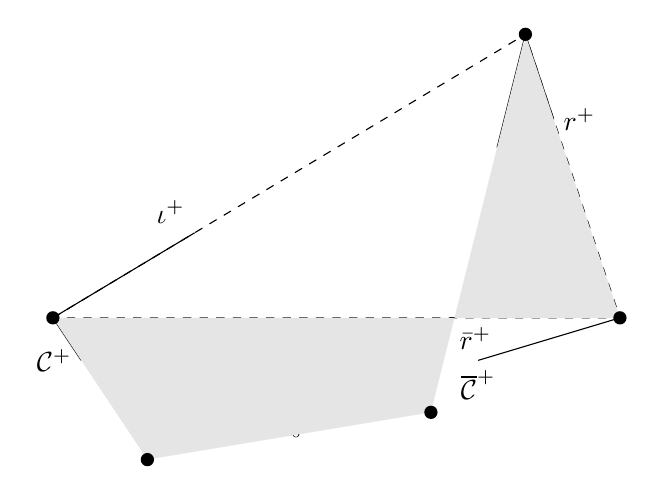
\begin{tikzpicture}[scale=1.2]
    % Define coordinates for the vertices
    \coordinate (A) at (0, 0);
    \coordinate (B) at (5, 3);
    \coordinate (C) at (6, 0);
    \coordinate (D) at (1, -1.5);
    \coordinate (E) at (4, -1);

    % Draw the outer dashed line
    \draw[dashed] (A) -- (B) -- (C) -- cycle;
    
    % Draw the inner solid lines
    \draw (A) -- ($(A)!0.3!(B)$) node[above left] {$\iota^+$};
    \draw (B) -- ($(B)!0.3!(C)$) node[right] {$r^+$};
    \draw (C) -- ($(C)!0.3!(A)$) node[below right] {$\bar{r}^+$};
    \draw (A) -- ($(A)!0.3!(D)$) node[left] {$\mathcal{C}^+$};
    \draw (B) -- ($(B)!0.3!(E)$) node[right] {$\overline{\mathcal{C}}^+$};
    \draw (C) -- ($(C)!0.3!(D)$) node[below] {$\overline{\mathcal{C}}^+$};

    % Draw the inner curves
    \draw[bend left] (D) to node[above] {$\Sigma^{T}$} (E);
    \draw[bend right] (E) to node[below] {$\Sigma^{T}_{r_0}$} (D);

    % Draw the shaded area
    \fill[black!10] (A) -- ($(A)!0.3!(D)$) -- (D) -- ($(D)!0.3!(E)$) -- (E) -- ($(E)!0.3!(B)$) -- (B) -- ($(B)!0.3!(C)$) -- (C) -- ($(C)!0.3!(A)$) -- cycle;

    % Mark the points with circles
    \foreach \point in {A,B,C,D,E} {
        \fill (\point) circle (2pt);
    }
\end{tikzpicture}

\end{document}